\documentclass[border=8pt]{standalone}
\usepackage{amsmath}
\usepackage{tikz}
\usetikzlibrary{arrows.meta,positioning,calc}
\begin{document}
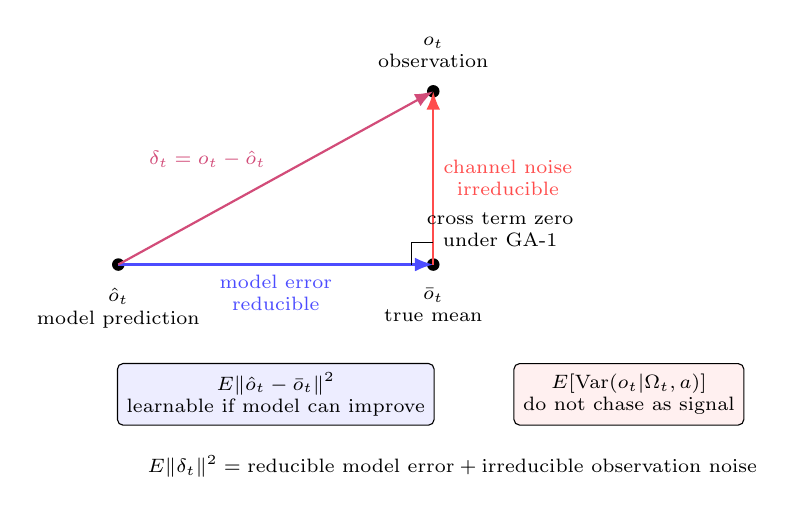
\begin{tikzpicture}[
  point/.style={circle, fill=black, inner sep=1.6pt},
  label/.style={align=center, font=\scriptsize},
  box/.style={draw, rounded corners=2pt, align=center, minimum width=2.65cm, minimum height=0.78cm, font=\scriptsize},
  arr/.style={-Latex, thick},
  brace/.style={decorate}
]

\coordinate (pred) at (0,0);
\coordinate (truth) at (4,0);
\coordinate (obs) at (4,2.2);

\node[point] at (pred) {};
\node[point] at (truth) {};
\node[point] at (obs) {};

\node[label, below=0.18cm of pred] {$\hat o_t$\\model prediction};
\node[label, below=0.18cm of truth] {$\bar o_t$\\true mean};
\node[label, above=0.18cm of obs] {$o_t$\\observation};

\draw[arr, blue!70] (pred) -- node[below, font=\scriptsize, align=center] {model error\\reducible} (truth);
\draw[arr, red!70] (truth) -- node[right, font=\scriptsize, align=center] {channel noise\\irreducible} (obs);
\draw[arr, purple!70] (pred) -- node[above left, font=\scriptsize] {$\delta_t=o_t-\hat o_t$} (obs);

\draw (3.72,0) -- (3.72,0.28) -- (4,0.28);
\node[label] at (4.85,0.45) {cross term zero\\under GA-1};

\node[box, fill=blue!7, below=1.25cm of $(pred)!0.5!(truth)$] (term1)
  {$E\|\hat o_t-\bar o_t\|^2$\\learnable if model can improve};
\node[box, fill=red!6, right=1.0cm of term1] (term2)
  {$E[\mathrm{Var}(o_t|\Omega_t,a)]$\\do not chase as signal};

\node[label, below=0.65cm of $(term1)!0.5!(term2)$]
  {$E\|\delta_t\|^2 = \text{reducible model error} + \text{irreducible observation noise}$};

\end{tikzpicture}
\end{document}
